% !TEX program = xelatex
\documentclass{book}
\usepackage{fancyvrb}
\usepackage{amsthm,amssymb,amsmath,amsfonts}
\usepackage{subfigure}
\usepackage{graphicx}
\usepackage{hyperref}
\usepackage{makeidx}
\usepackage{color}
\makeindex
\renewcommand{\baselinestretch}{1.5} 
\addtolength{\oddsidemargin}{-.875in}
\addtolength{\evensidemargin}{-.875in}
\addtolength{\textwidth}{1.75in}

\addtolength{\topmargin}{-.875in}
\addtolength{\textheight}{1.75in}

\usepackage{xepersian}
\settextfont{XB Niloofar}
\author{پویا آقاحسینی}
\title{طراحی هندسی کامپیوتری صفحات ۱-۳۰}
\begin{document}
	\maketitle
	\tableofcontents
	\listoffigures
	\listoftables
	\chapter*{پیش‌گفتار}
	\addcontentsline{toc}{chapter}{پیش‌گفتار}
	\begin{flushright}
		
		هندسه محاسباتي يا به تعبير فرانسوی‌ها هندسه آلگوريتمي 
		\footnote{\lr{Geometrie algorithmique}}
		از دهه هفتم قرن نوزدهم به صورت يک رشته تحقيقاتي مستقل رسما متولد شد. اگر چه تولد اين رشته جديد را به پايان نامه دکتري ميشل شاموس
		\footnote{\lr{Michael Shamos}}
		که بعداً با نام مشترک خود وي و
		استادش پاراپرتا
		\footnote{\lr{Franco P.Preparata}}
		به صورت اولين کتاب در زمينه هندسه محاسباتي منتشر شد
		\footnote{\lr{Computational Geometry - An Introduction}}
		ربط مي دهند، ولي تحقيق و پژوهش در مورد
		بسياري از مفاهيم اساسي اين رشته از قبيل دياگرام ورونوي، مثلث بنديها . . . به سده‌هاي قبل‌تر بر ميگردد.
\end{flushright}
	\begin{flushright}
	
	هندسه محاسباتي در طول عمر رسمي کمتر از 50 ساله خود، با گسترش بسيار زياد، نظرات پژوهشگران و محققان بسياري را
	بهخود جلب کرده است. طرح مسائل بسيار زيبا که صورت ساده و قابل فهمي دارند و کاربردهاي بسيار گسترده در اکثر علوم
	مهندسي، کامپيوتر، رباتيک، جغرافيا، بايوانفورماتيک، مدل سازي . . . از يک سو، و ارائه راه حل هاي الگوريتمي و قابل پياده سازي و اجرا توسط ماشين و نيز بکارگيري قوتها و توانائي هاي آلگوريتم، ساختمان داده ها و هندسه تئوريک از سوي ديگر
	هندسه محاسباتي را به يک رشته تحقيقاتي مدرن، به روز و پرجاذبه تبديل کرده است.
\end{flushright}
	\begin{flushright}
اگر چه بسياري از مسائل هندسه محاسباتي سخت و پر چالش هستند ولي معمولاً صورت آنها ساده و قابل فهم است. به همين دليل همچون يک اقيانوس عميق در عين حال با سواحل کم عمق و زيبا، براي محققان و پژوهشگران بسيار جذاب مي باشد.	
\end{flushright}
	\begin{flushright}
کاربردهاي هندسه محاسباتي بسيار گسترده است. چندان دور از واقعيت نيست اگر ادعا کنيم؛ هندسه محاسباتي اين توانائي را دارد که براي بسياري از مشکلات و مسائل در زمينه‌هاي مهندسي و کاربردي با روش هاي الگوريتمي يک مدل درست کند. اگر چه هميشه حل اين مدل به سادگي صورت نمي پذيرد.\\	
\end{flushright}
	\begin{flushright}
	و اما از سوي ديگر طراحي و تحليل آلگوريتم براي دانشجويان علوم و مهندسي کامپيوتر و حتي رياضي، اصلي و پايه اي ترين درس در دوره ي کارشناسي است. دانشجوياني که اين درس را به خوبي فرا مي گيرند در مشاغل مختلف مهندسي و برنامه نويسي در کار با کامپيوتر مهارت خواهند داشت. بنابراين بالا بردن مهارت دانشجويان در زمينه طراحي و تحليل آلگوريتم براي دانشکده هاي رياضي و علوم و مهندسي کامپيوتر بسيار مهم و استراتژيک مي باشد.\\
\end{flushright}
	\begin{flushright}
	مسائل کتاب حاضر بارها در مقطع کارشناسي و بعضاً کارشناسي ارشد در دانشکده رياضي و علوم کامپيوتر تدريس شده است، و به عنوان يک درس کمکي براي فراگيري مفاهيم و روشهاي طراحي و تحليل الگوريتم با کمک مثال هايي از هندسه مفيد مي باشد.\\
\end{flushright}
	\begin{flushright}
	
	در واقع مباحث اين کتاب نه مي تواند جايگزين درس طراحي و تحليل الگوريتم شود، که از کليت مباحث درس طراحي الگوريتم برخوردار نيست و نه مي تواند جايگزين درس هندسه محاسباتي شود، که تمام مباحث آن را پوشش نمي دهد. بلکه کتاب حاضر به عنوان مرجع درسي با نام "هندسه آلگوريتمي" و يا "آگلوريتم هاي هندسي" و به منظور تقويت درک دانشجويان از مباحث طراحي الگورتيم  و نيز آشنائي با مسائل هندسه محاسباتي براي دانشجويان سال آخر دوره‌ي کارشناسي و يا سال اول کارشناسي ارشد علوم و مهندسي کامپيوتر قابل ارائه مي باشد.\\
\end{flushright}
	\begin{flushright}
		در کتاب پيش روي به بهانه آموزش طراحي و تحليل آلگوريتم ها مثال هاي جذاب و زيبائي از هندسه محاسباتي طرح و حل مي‌شود. بعضي از مسائل از مقالات و آخرين تحقيقات روز انتخاب شده است و دانشجويان را با مرزهاي دانش آشنا مي شوند. و بعضي ديگر از کتب رايج هندسه محاسباتي.
\end{flushright}
	\begin{flushright}
		واقعيت اين است که اين کتاب بيشتر يک کتاب تحليل الگوريتم و روش‌هاي حل مسئله است تا بررسي ساختمان داده‌ها. دليل آن اين است که در حل مسائل عمدتا به تحليل آلگوريتم پرداخته شده است و از مباحث ساختمان داده‌ها نسبتا سطحي عبور کرده‌ايم.
\end{flushright}
	\begin{flushright}
	در حقيقت پرداختن به تحليل و الگوريتم و بررسي ساختمان داده‌ها بطور هم زمان مقداري موجب خلط مباحث مي‌شود، و خواننده نه به درستي با روش ها و آلگوريتم‌هاي حل مسئله آشنا مي‌شود و نه با شيوه‌هاي انتخاب و تحليل ساختمان داده‌ها.
\end{flushright}
	\begin{flushright}
		به همين دليل در اين کتاب ترجيح داده ام که بررسي آلگوريتم‌ها را انتخاب کنم و تحليل ساختمان داده‌ها را به فرصتي ديگر احاله دهيم.
\end{flushright}

\chapter{مقدمه}
در اين فصل بطور مختصر به بررسي چند سؤال ابتدايي ولي بسيار مهم مي‌پردازيم.\\
\\
به اين سؤالات معمولا در درس ساختمان داده‌ها و طراحي آلگوريتم مقدماتي به تفصيل پاسخ داده مي‌شود. در اينجا نيز به منظور يادآوري، به شکلي بسيار مختصر به آنها مي‌پردازيم. اين سؤالات عبارتند از:
\begin{itemize}
	\item
	نوع داده مجرد چيست و چه استفاده اي دارد؟
	\item 
	ساختمان داده ها چيست و چه کاربردي دارد؟
	\item 
	آلگوريتم چيست؟
\item 
	مفهوم آناليز آلگوريتم به چه معني است؟
	\item
	مسئله محاسباتي به چه نوع مسئله اي مي گوييم؟
\end{itemize}
	\section*{نوع داده مجرد‌}
	\addcontentsline{toc}{section}{نوع داده مجرد‌}
	يک نوع داده مجرد  
	\footnote{\lr{  Abstract Data Type- ADT}}
	يك مدل رياضي براي داده‌ها است كه تعدادي عمليات روي آن تعريف مي‌شود. بنابراين هر نوع داده مجرد متشكل است از مجموعه‌اي از مقادير (داده‌ها) و مجموعه‌اي از عمليات بر روي آن‌ها. اين مجموعه داده‌ها و عمليات روي آن، يك ساختار رياضي تشكيل مي‌دهد که با كمك آن يك ساختمان داده‌ها
	\footnote{\lr{Data Structure}
		 همواره ساختمان داده ها ترجمه شده است. لاکن اخيرا بعضي همکاران ترجمه داده ساختار را صحيح تر دانسته اند. از آنجا که در ادبيات ترجمه ساختمان داده ها بيشتر بکار رفته است و تقريبا رايج شده است ما نيز از اين کلمه استفاده مي کنيم.
	}
	  پياده‌سازي مي‌شود.\\
	يک نوع داده مجرد‏ شامل تعدادي عملگر است. اين عملگرها توسط آلگوريتم بکار گرفته مي‌شوند. بنابراين براي هر يک نوع داده مجرد، ‏دسته‌اي از عملگرها وجود دارد.\\
	يك مثال ساده از داده‌هاي مجرد مي تواند مجموعه اعداد صحيح با عملگرهاي (+,-,×,\%,/)   باشد.\\
	آرايه، مثال ساده يك-بعدي از يک نوع داده مجرد‏ مي‌باشد كه بصورت زير تعريف مي‌شود:
	\begin{itemize}
		\item
مجموعه عناصر: دنباله‌اي با طول ثابت (مجموعه‌اي مرتب) از عناصر كه همگي از يك نوع اند.
		\item 
عمليات اصلي: دست‌يابي مستقيم به هر عنصر آرايه، طول آرايه
	\end{itemize}	
به عنوان مثال‌هايي براي يک نوع داده مجرد مي توان: صف، ليست، صف اولويت، مجموعه، درخت، دنباله نام برد.\\
ساختمان داده‌ها يک مدل براي سازماندهي داده‌ها است. ساختمان داده‌ها عبارت است از ساختن تعدادي بلوک که بخش‌هاي يک آلگوريتم را بهم متصل مي‌کند، برکارايي آلگوريتم تاثير مي‌گذارد و براي اجراي يک آلکوريتم سهولت ايجاد مي‌کند. به همين دليل يادگيري ساختمان داده‌ها بسيار اساسي و مهم است.\\
ساختمان داده‌ها يک روش براي ساخت، تغيير و دسترسي به داده‌ها است. به تعبيري رسمي‌تر، ساختمان داده‌ها عبارت است از سه مؤلفه: 
	\begin{enumerate}
	\item
يک ساختار پايدار که داده‌هاي مجرد در آن نگهداري مي‌شوند.
	\item 
مجموعه‌اي از عملگرها براي بکارگيري نوعي خاص از داده‌هاي مجرد
	\item 
اجراي عملگرهاي تعريف شده بر روي داده‌ها و ساختارهاي نگهداري‌شده 
{\colorbox{yellow}{(ادامه صفحه 24 کتاب نوشته شود.)}}
\end{enumerate}	
 ساختمان داده‌ها را به طور مختصر مي‌توان بصورت زير دسته‌بندي كرد:
\begin{enumerate}
	\item
	 	ساختارهای خطی
	 	\footnote{\lr{Linear Structures}}
	 	\begin{enumerate}
	 		\item 
	 		لیست های فشرده
	 		\footnote{\lr{Dense Lists}}
	 		:
	 		\begin{enumerate}
	 			\item 
	 			رشته‌ها
	 				 	\footnote{\lr{Strings}}
	 			\item 
	 			آرایه‌ها
	 				 				 	\footnote{\lr{Arrays}}
	 			\item 
	 			پشته‌ها
	 				 				 	\footnote{\lr{Stacks}}
	 			\item 
	 			صف‌ها
	 				 				 	\footnote{\lr{Queues}}
	 		\end{enumerate}
 			\item 
 			لیست‌های پیوندی
 				 				 	\footnote{\lr{Linked Lists}}
 			\begin{enumerate}
 				\item 
 			انواع ليستهاي يك طرفه و دو طرفه و مدور
 			  	\item 
 			پشته و صف به روش ليستهاي پيوندي 
 			
 			\end{enumerate}
	 	\end{enumerate}
 	\item 
 	ساختارهای غیر‌خطی
 		 				 	\footnote{\lr{Non-Linear Structures}}
 	\begin{enumerate}
 		\item
 		گراف‌ها
 			 				 	\footnote{\lr{Graphs}}
 		\item 
 		درخت‌ها
 			 				 	\footnote{\lr{Trees}}
 	\end{enumerate}
\end{enumerate}
\section*{مسئله محاسباتی}
	\addcontentsline{toc}{section}{مسئله محاسباتی}
يک مسئله محاسباتي مسئله‌اي است که مي‌توان آن‌ را با کمک يک مجموعه از دستورات پي در پي رياضي نوشت و سپس توسط کامپيوتر حل نمود. البته توجه داشته باشيد که بعضي مسائل محاسباتي هستند که توسط کامپيوتر قابل حل نيستند؛ مانند يافتن يک دور بسته با حداقل طول که از تمام نقاط يک مجموعه داده شده دقيقا يک بار  بگذرد.)\\
بنابراين، يک مسئله محاسباتي مي‌تواند بصورت مجموعه‌اي از دستورات نوشته شود؛ براي هر دستور يک راه حل وجود دارد و قابل پياده‌سازي مي‌باشد. \\
يک مسئله محاسباتي داراي يک ورودي است و يک خروجي که وابسته به ورودي مي باشد.\\
مثال1:  عدد$n$ داده شده است. بررسي کنيد اين عدد اول است يا خير.\\
در اين مثال عدد صحيح $n$ ورودي است و پاسخ بله يا خير که مي توان بجاي آن صفر و يک در نظر گرفت به عنوان خروجي \\
مثال2: مجموعه‌اي از نقاط در صفحه داده شده است. يک چندضلعي ساده با کمک اين نقاط بسازيد.\\
در اين مسئله محاسباتي مجموعه اي از نقاط صفحه ورودي مسئله است و يک چندضلعي ساده که با کمک نقاط ورودي ساخته شده خروجي مسئله.   \\
براي حل يک مسئله محاسباتي، به يک نوع داده مجرد، يک ساختمان بر روي آن و مجموعه‌اي از عملگرها که ساختمان مربوطه از اين عملگرها پشتيباني کند، نياز داريم. استفاده از اين عملگرها به حل مسئله توسط ماشين مي‌انجامد. 
\section*{حل مسئله کامپیوتری}
	\addcontentsline{toc}{section}{حل مسئله کامپیوتری}
حل مسئله توسط کامپيوتر، يکي از مهارت‌هاي ارزشمند است که مي‌تواند يکي از اهداف اصلي دانش علوم کامپيوتر باشد و دانشجوي علوم کامپيوتر بايستي آن‌ را در دوران تحصيل خود کسب کند. در حقيقت توانايي حل مسائل مختلف توسط کامپيوتر مي‌تواند مهارت اصلي يک دانش‌آموخته رشته علوم کامپيوتر تلقي شود. که طبيعتا مهارت ارزشمندي نيز مي باشد.\\
امروزه عمدتا با مسائلي سر و کار داريم که از داده‌هاي حجيم استفاده مي‌کنند؛ بنابراين نه تنها بايد براي حل آنها از روش‌هاي کامپيوتري استفاده نمود ، بلکه بايد در مورد سازماندهي داده‌ها نيز بررسي‌هاي لازم را انجام داد. از سوي ديگر، بسياري از مسائل، يکبار پيش‌پردازش مي‌شوند؛ ولي بارها و بارها براي داده‌هاي مختلف مورد سؤال قرار مي‌گيرند. در اين گونه مسائل، سرعت در پاسخ داده بسيار مهم است. بنابراين حل اين گونه مسائل نه تنها با کامپيوتر، بلکه با روش‌هاي کامپيوترهاي بسيار سريع بايد صورت پذيرد و زمان در حل اين گونه مسائل بسيار مهم است. يک دانش آموخته علوم کامپيوتر مي‌بايست لوازم ضروري اين مهارت را داشته باشد. يکي از اين لوازم، طراحي آلگوريتم خصوصا آلگوريتم‌هاي هندسي مي باشد.\\
\section*{مدل‌سازی}
	\addcontentsline{toc}{section}{مدل‌سازی}
براي حل يک مسئله توسط کامپيوتر بايد مسئله در قالب يک مدل در آيد که با سازوکارهاي کامپيوتر قابل درک باشد؛ لذا بايد براي آن يک مدل ساخت و يا به عبارت ديگر، بايد آن‌ را مدل‌سازي کرد. براي اين کار، بايد پارامترهاي اصلي مسئله را شناخت و از آن‌ها براي تعريف مدل‌ مسئله استفاده نمود.\\
اگر بتوان مدل‌هاي اصلي مسئله را به کار گرفت، مي توان مدل مسئله را ساده کرد و آنگاه حل مسئله نيز ساده‌تر خواهد شد. براي مدل‌سازي بايستي پارامترهاي جزئي تا حد ممکن ناديده گرفت و پارامترهاي اصلي را تعيين و برد.\\
براي حل مدل مسئله بايد از يک آلگوريتم استفاده کرد. اين الگوريتم مشخص مي‌کند که داده‌هاي مسئله بايد توسط چه ساختمان داده اي بيان شوند و روي اين ساختمان داده چه اعمالي صورت گيرد.
\section*{مراحل حل یک مسئله}
	\addcontentsline{toc}{section}{مراحل حل یک مسئله}
\begin{itemize}
	\item
	بيان مسئله 
	\footnote{\lr{Problem Statement}}
	که عبارت است از تعريف صورت مسئله به شکلي واضح و دقيق و تعيين ورودي و خروجي
	\item 
	تدوين يك مدل
		\footnote{\lr{Modeling}}
	 که عبارت است از تدوين يک مدل مناسب براي مسئله، حذف پارامترهاي غيرضروري که امکان حذف آنها وجود دارد و تعيين پارامترهاي اصلي.\\
	 
	 براي مدل سازي يک مسئله معمولا دو سؤال مطرح مي شود که پاسخ به آنها به تدوين يک مدل مناسب براي مسئله منجر خواهد شد.
	 \begin{itemize}
			\item 
			براي مدل‌سازي يک مسئله، راه حل اول که ساده‌تر به نظر مي‌رسد، اين است که مسئله ديگري مشابه آن بيابيم و با اعمال تغييراتي که لازم است، آن‌ را تبديل به مدلي براي حل مسئله خودمان کنيم. براي استفاده از اين روش بايد اطلاعات خود را در مورد مدل‌هاي مختلف حل مسئله و نمونه هاي مسائلي که مدل و حل شده است افزايش دهيم.
			\item 
			روش ديگر اين است که مستقيما تا حد ممکن پارامترهاي مسئله را ساده و سپس براي آن يک مدل طراحي کنيم.  بخش اول اين کار را ساده‌سازي مسئله مي‌گويند. يعني تبديل مسئله سخت با پارامترهاي متعدد به مسئله‌اي ساده با پارمترهاي اندک. هرچه ساده‌سازي مسئله بهتر صورت پذيرد، طراحي مدل براي آن ساده‌تر خواهد بود. براي اينکار لازم است مسئله و پارمترها بطور دقيق آناليز شوند و ميزان  تأثير پارامترها در پاسخ مسئله معين گردد.
	 \end{itemize}
\end{itemize}
\section*{آلگوریتم}
	\addcontentsline{toc}{section}{آلگوریتم}
تعاريف متعددي در مورد آلگوريتم وجود دارد. در يک تعريف ساده مي توان گفت: \\
آلگوريتم عبارت است از يک روش براي حل يک مسئله محاسباتي. يا آلگورتيم عبارت است از مجموعه‌اي متناهي از قواعد و دستورات كه مراحل حل يك مسئله توسط کامپيوتر را بيان مي‌كند.\\
براي انجام هر نوع پردازش در كامپيوتر آلگوريتم لازم است؛ لذا از اين ديدگاه، علم كامپيوتر يعني طراحي و تحليل آلگوريتم.\\
يک آلگوريتم را مي‌توان به روش‌هاي مختلف بيان و دستورات آن را با کمک کامپيوتر محاسبه کرد. آلگوريتم و ساختمان داده‌ها با يکديگر ارتباط متقابل دارند. آلگوريتم، ساختمان داده‌ها را انتخاب مي‌کند و عملگرهاي آن‌ را بكار مي‌گيرد. ساختمان داده‌ها مانند بلوک‌هايي هستند که مراحل آلگوريتم با کمک آن‌ها ساخته مي‌شود. يك آلگوريتم بايد از سادگي و قطعيت برخوردار باشد تا بتواند توسط کامپيوتر اجرا شود. يك آلگوريتم به زباني كه براي ماشين قابل فهم است، ترجمه و پياده سازي مي‌شود. اين عمل را اجراي آلگوريتم گويند.\\
اکنون به طرح چند سؤال و پاسخ مختصر آن مي پردازيم. اگر پاسخ ها بسيار کلي و سريع به نظر رسيد و نتوانست شما را متقاعد کند بايد به کتب طراحي الگوريتم مراجعه نماييد.
\section*{چند سؤال و جواب اوليه}
	\addcontentsline{toc}{section}{چند سؤال و جواب اوليه}
\begin{itemize}
	\item 
يك آلگوريتم را چگونه طراحي كنيم؟\\
طراحي آلگوريتم يک علم و در عين حال يک هنر است که با حل مسئله و نيز تجربه بدست مي‌آيد. در اين کتاب سعي مي‌شود بعضي از روش‌هاي مرسوم مورد بررسي قرار گيرد و با حل نمونه هاي متعدد، اين مهارت افزايش يابد.
\item 
درستي يك آلگوريتم به چه معني است؟   \\
درستي يک آلگوريتم بدين معني است که آلگوريتم بايد بتواند تمام نمونه‌هاي مسئله را حل کند. بعضي مواقع براي اثبات درستي يک آلگوريتم اثبات لازم است. بعضي مواقع نيز آلگوريتم بازگوکننده مراحل يک مسئله است و اثبات درستي، در خود راه حل مسئله مستتر مي‌باشد.
\item 
چگونه يك آلگوريتم را تجزيه و تحليل كنيم؟  \\
مسئله تجزيه و تحليل يک آلگوريتم، مسئله مهمي است که نتيجه آن ارزشيابي آلگوريتم‌ها مي‌باشد. با تجريه و تحليل يک الگوريتم، کارايي آن مشخص مي‌شود.
\item 
عملي‌بودن يك آلگوريتم را چگونه بررسي كنيم؟   \\
عملي‌بودن يک آلگوريتم با پياده‌سازي آن قابل بررسي است.اگر آلگوريتمي قابل پياده‌سازي بود و توانست نمونه‌هاي مسئله مربوطه را حل کند، براي حل مسئله يک روش عملي ارائه داده است.
\end{itemize}
بنابراين براي حل مسئله ابتدا طراحي يک مدل لازم است که مانند يک الگو به بررسي، تحليل و حل مسئله کمک مي کند. سپس طراحي يك آلگوريتم در آن مدل و استفاده از ساختمان داده مناسب براي پياده سازي آلگوريتم. اثبات درستي و صحت آلگوريتم و تجزيه و تحليل آلگورتيم مراحل مهمي است که بدنبال طراحي آلگوريتم بايستي مد نظر قرار گيرد. در بخش هاي زير در مورد اين مفاهيم توضيحات بيشتري خواهيم داد.
\section*{طراحی آلگوریتم‌ها}
	\addcontentsline{toc}{section}{طراحی آلگوریتم‌ها}
ساختار و مراحل مقدماتي طراحي يك آلگوريتم را به صورت زير مي‌توان بيان نمود.\\
\begin{enumerate}
	\item 
	مراحل ورودي 
	\footnote{\lr{Input Step}}
	تعيين ورودي آلگوريتم که بايستي دقيق، معين و قابل بررسي باشد. 
	
	مرحله جايگذاري
		\footnote{\lr{Assignment Step}}
	 تعريف تعدادي زيرمسئله براي حل مسئله اصلي، چينش دقيق زيرمسائل و تبيين يک مدل و استراتژي براي ورورد به مسئله
	\item 
	مرحله تصميم‌گيري 
		\footnote{\lr{Decission Step}}
	انتخاب يک مسير اصلي براي حل مسئله يا به عبارت ديگر طراحي يک استراتژي از قبيل حريصانه، تقسيم و حل، بازگشت به عقب و .... براي حل مسئله
	\item 
	مرحله تكرار 
		\footnote{\lr{Iteration Step}}
	ممکن است براي حل مسئله نياز به بررسي و تکرار حل زير مسائل باشد.
	\item 
	مرحله خروجي 
		\footnote{\lr{Output Step}}
	لازم است مسئله يک خروجي نهايي مشخص داشته باشد که در انتها به آن اشاره مي شود. 
\end{enumerate}
يك آلگوريتم بايد داراي ويژگي هاي زير باشد.
 \lr{(Knuth-1973)}\\
\begin{enumerate}
	\item 
	متناهي بودن 
			\footnote{\lr{Finiteness}}
	آلگوريتم بايستي در زماني قابل قبول تمام شود و کار حل مسئله به انتها برسد.  
	\item 
	معين بودن 
			\footnote{\lr{Definiteness}}
	يك آلگوريتم بايد بدون ابهام، قطعي و در هر مرحله واضح و روشن باشد.
		\item 
	كليت 
			\footnote{\lr{Generality}}
			تمام حالات خاص مسائل را در بر بگيرد.
		\item 
	كارايي
			\footnote{\lr{Effectiveness}}
			 آلگوريتم بايد تمام نمونه هاي مسئله را به درستي حل کند.
		\item 
	ورودي 
			\footnote{\lr{Input}}
			يك آلگوريم بايستي داراي يک ورودي باشد.
		\item 
	خروجي 
			\footnote{\lr{Output}}
			يك آلگوريتم بايد كاري انجام دهد و خروجي داشته باشد.
\end{enumerate}
\section*{آنالیز یک آلگوریتم}
	\addcontentsline{toc}{section}{آنالیز یک آلگوریتم}
پس از طراحي يک آلگوريتم براي حل يک مسئله، همواره يک سؤال مطرح است: "آيا آلگوريتم بهتري براي حل مسئله وجود دارد؟" \\
به عبارت ديگر، براي حل هر مسئله ممکن است تعدادي آلگوريتم وجود داشته باشد. سؤال اين است که "کدام آلگوريتم براي حل مسئله مناسب‌تر است؟"
آناليز يک آلگوريتم، عبارت است از اندازه‌گيري کارايي آن؛ بدين معني که يک آلگوريتم تا چه حد و چه موقع قابل اجرا است و اجراي آن به چه ميزان منابع نياز دارد. همچنين زمان و حافظه مورد نياز آلگوريتم به صورت تابعي از اندازه ورودي الگوريتم بايد بررسي گردد. با کمک آناليز آلگوريتم، کارآيي ساختمان داده‌هاي مورد نياز تعيين مي‌شود. مي‌توان زمان موثر دو آلگوريتم براي حل يک مسئله را مقايسه کرد و بدين روش، الگوريتم‌ها مقايسه و رتبه‌بندي مي‌شوند.\\
يک روش ساده براي مقايسه آلگوريتم‌ها، اجرا و سپس مقايسه آنها است؛ اگرچه مقايسه زمان اجراي آلگوريتم‌ها خود مشکلاتي دارد و سؤلات متعددي را به دنبال دارد. از جمله اينکه:\\
\begin{itemize}
	\item 
	چه داده‌اي مورد استفاده قرار گيرد.
	\item 
	چه کامپيوتري براي اجرا در نظر گرفته شود.
	\item 
	آلگوريتم با چه زبان برنامه نويسي نوشته شود.
\end{itemize}
بنابراين باتوجه به وجود پارمترهاي متعدد که هريک در اجرا و سرعت و نيز ميزان استفاده از فضاي حافظه کامپيوتر تاثيردارد مقايسه آلگوريتم‌ها کار خيلي ساده‌اي نيست.	\\

براي آناليز يک آلگوريتم لازم است کارآيي آن مورد بررسي قرار گيرد. با بررسي کارآيي يک آلگوريتم مشخص مي‌شود که الگوريتم چه موقع قابل استفاده خواهد بود. از سوي ديگر، آناليز آلگوريتم‌هاي مختلف، امکان مقايسه و درجه‌بندي آنها را در هنگام حل يک مسئله واحد فراهم مي‌آورد.\\
آناليز يک آلگوريتم بطور کلي به معني بررسي دو نکته در مورد آلگوريتم است: فضا (حافظه) و زمان مورد نياز آلگوريتم در هنگام حل يک مسئله. در اين کتاب، عمدتا به  زمان مورد نياز يک آلگوريتم براي حل يک مسئله توجه خواهد شد.\\
به منظور محاسبه زمان يك آلگوريتم، لازم است عملگرها و تعداد تكرار آنها مورد بررسي قرار گيرد. به عنوان مثال، در بررسي مسئله محاسبه پوش محدب چند ضلعي، رؤس چند ضلعي را ورودي مسئله در نظر مي گيريم و تعداد دفعاتي كه اضلاع چندضلعي مورد مراجعه قرار مي‌گيرند، به عنوان زمان آلگوريتم محاسبه مي‌شود. به عنوان مثال ديگر، در مرتب سازي و جستجو، هنگامي که يک آرايه از اعداد به صورت ورودي مسئله مورد نظر قرار مي‌گيرد، تعداد دفعاتي که اعداد بررسي و يا مقايسه مي‌شوند، به عنوان زمان آلگوريتم محاسبه مي‌شود. زمان كلي يك آلگوريتم برابر است با مجموع زمان مراحل اجراي آن. اين زمان با کمک محاسبه مجموع زمان مورد نياز براي انجام عملگرهاي آلگوريتم مشخص مي‌شود.\\
از آنجا كه زمان اجرا بستگي به مدل محاسبه دارد و نمي‌تواند به کامپيوتر و وسايل سخت‌افزاري ديگر متکي باشد، بنابراين بايد مدل واحدي را براي محاسبه آلگوريتم‌هاي متفاوت در حل يك مسئله به كار برد.  اين مدل که قاعدتا بايد مستقل از نوع و مدل و توانايي کامپيوتر باشد، پيچيدگي زمان الگوريتم ناميده مي‌شود.
\section*{مقایسه کران بالا و کران پایین}
	\addcontentsline{toc}{section}{مقایسه کران بالا و کران پایین}
آناليز آلگوريتم، علاوه بر تعيين کران بالا و کران پائين، زمان حل يک مسئله توسط آن آلگوريتم را نيز تعيين مي‌کند. هنگامي که کران بالا و کران پائين زمان مسئله را داشته باشيم، آن‌ها را با هم مقايسه مي‌کنيم و ميزان مفيد بودن آلگوريتم را مي‌سنجيم. با محاسبه پيچيدگي حد بالا مي توان به اين سوال پاسخ داد که آيا آلگوريتم براي حل تمام نمونه‌هاي مسئله مناسب است يا خير. همچنين محاسبه پيچيدگي حد بالا نيز نشان مي‌دهد که آلگوريتم براي حل کدام نمونه از مسائل مي‌تواند ارزشمند باشد. 
\section*{اعتبارسنجی آلگوریتم}	\addcontentsline{toc}{section}{اعتبارسنجی آلگوریتم}
اعتبار سنجي آلگوريتم عبارت است از نشان‌دادن اينکه آلگوريتم براي کليه ورودي‌هاي داده شده صحيح عمل مي‌کند يا خير. براي سنجش اعتبار آلگوريتم، معمولا نمونه‌هاي خيلي خاص مسئله در نظر گرفته مي‌شود و توانايي آلگوريتم در حل اين نمونه‌ها مورد تحليل قرار مي‌گيرد.\\
پس از نهايي‌شدن اين مراحل، مي‌توان با استفاده از يک زبان برنامه نويسي مناسب، الگوريتم را پياده‌سازي کرد.
\chapter{ساختمان داده‌های هندسی}
كوچكترين شيء هندسي، نقطه است. يک رابطه يك به يك بين نقاط در صفحه و زوج‌هاي مرتب $(x,y)$ وجود دارد؛ به اين صورت که يك نقطه را در صفحه مي‌توان با زوج مرتب $(x,y)$ نمايش داد. همچنين زوج مرتب $(x,y)$ مي‌تواند به عنوان يك بردار در صفحه نيز در نظر گرفته شود. در حقيقت مبداْ ابتداي اين بردار و نقطه $(x,y)$  انتهاي آن خواهد بود. با اين تعبير، يک بردار، يك پاره‌خط جهت‌دار است که از مبداْ به سمت نقطه $(x,y)$ امتداد دارد. مبداْ مختصات يعني نقطه $(0,0)$‌ بردار صفر ناميده و با $0$ نشان داده مي‌شود.
\section*{عملگرهای روی بردارها}	\addcontentsline{toc}{section}{عملگرهای روی بردارها}
مي‌توان روي بردارها که به صورت فوق تعريف شدند، تعدادي عملگر تعريف نمود.\\

عملگر جمع : اگر
$\vec{a} = (x_{1},y_{1})$
و
$\vec{b} = (x_{2},y_{2})$
آنگاه  عملگر جمع ‏را بصورت 
$\vec{a}+\vec{b} = (x_{2}+x_{2},y_{1}+y_{2})$
 تعريف مي‌کنيم.\\
 
 از نظر هندسي، با کمک بردارهاي 
 $\vec{a}$
 و
 $\vec{b}$
  مي‌توان يک متوازي‌الاضلاع ساخت که
   $\vec{a}+\vec{b}$
قطر آن را تشكيل مي‌دهد.\\

 عملگر ضرب عددي:  اگر $t$ يك عدد حقيقي باشد، آنگاه تعريف مي‌كنيم: 
 $t\vec{a} = (tx,ty)$
 \\

 اگر
 $t>0$
  آنگاه
   $\vec{ta}$
   و
    $\vec{a}$
  هم‌جهت خواهند بود؛ در غير اين صورت، جهت آن‌ها در خلاف جهت يكديگر مي‌باشد.\\

  عملگر تقاضل : اگر 
  $\vec{a} = (x_{1},y_{1})$
  و
  $\vec{b} = (x_{2},y_{2})$
  آنگاه  تعريف مي‌کنيم: 
  $\vec{a}+\vec{b} = \vec{a}+\vec{(-b)}$
  \\
  \\

  \textbf{
  	 پاره‌خط جهت‌دار $ab$ :
  	}
  عبارت است از پاره‌خطي که ابتداي آن ثابت و در نقطه $a$، انتهاي آن در نقطه $b$ و جهت آن نيز از $a$ به سمت $b$ باشد. \\
  سه نقطه$a$ و $b$ و $c$  را در نظر مي‌گيريم. گوييم مثلث
  $\triangle abc$ 
   که توسط اين سه نقطه ساخته مي‌شود، چرخش مثبت يا چرخش چپ (چرخش منفي يا چرخش راست) دارد؛ اگر و فقط اگر  نقطه $c$ سمت چپ (سمت راست) پاره‌خط جهت‌دار $ab$ باشد. 
   \begin{figure}[h]
   			\begin{center}
   			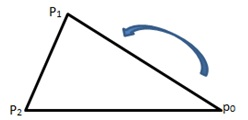
\includegraphics{1.jpg}
		   	\caption{شکل 1}
   		\end{center}
   	\label{شکل 1}
   \end{figure}
به عبارت ديگر، اگر  
$\theta_acb$
 زاويه‌اي باشد که از چرخش 
 $\vec{ca}$
 بصورت پادساعت گرد به سمت 
  $\vec{cb}$
  بدست آمده است، آنگاه مثلث   
  $\triangle abc$ 
   چپ گرد (راست گرد) است يا چرخش مثبت ( چرخش منفي) دارد؛ اگر و فقط اگر 
   $(180<\theta_{acb}<360)$  
      $(0<\theta_{acb}<180)$  
      \\
      
      اگر 
        $\vec{A}$
        و
                $\vec{B}$
      دو بردار باشند،
      $|A\times B|$
       برابر است با مساحت متوازي‌الاضلاع ساخته‌شده به وسيله دو بردار. \\
       
       به عبارت ديگر، اگر
       $\vec{A}= a - c$
       و
              $\vec{A}= b - c$
        آنگاه مساحت مثلث 
          $\triangle abc$ 
         عبارت است از نصف بردار
      $A\times B$
      \\
      \[
      \frac{1}{2}A \times B = \begin{vmatrix}
      i	& j & k \\
      a_{x} & a_{y} & a_{z}\\
      b_{x} & b_{y} & b_{z}
      \end{vmatrix} = (a_{x}b_{y} - a_{x}b_{y})i + (a_{x}b_{z} - a_{z}b_{x})j + (a_{x}b_{y} - a_{y}b_{x})k
      \]
      اگر اين بردارها در دو بعد باشند، آنگاه 
      $(b_{z}=a_{z}=0)$ 
      \\
      
      در اين صورت، حاصل‌ضرب دو بردار عبارت است از بردار نرمال صفحه مثلث حاصل از دو بردار.\\
      مقدار اين بردار برابر است با      
      $|A\times B|= (A_{0}B_{1} - A_{1}B_{0})$
      \\
      و اين برابر است با دترمينان زير:
      \[
      2 \times Area(a,b,c) = \begin{vmatrix}
      a_{4} & a_{y} & 1 \\
      b_{x} & b_{y} & 1 \\
      c_{x} & c_{y} & 1
      \end{vmatrix} = (b_{x} - a_{x})(c_{y} - a_{y}) - (b_{y} - a_{y})(c_{x} - a_{x})
      \]
      اگر مقدار اين دترمينان مثبت باشد، نقاط $a,b,c$ چپ‌گرد اند.\\
      اگر مقدار اين دترمينان منفي باشد، نقاط $a,b,c$ راست‌گرد اند.\\
      اگر مقدار اين دترمينان صفر باشد، نقاط $a,b,c$ هم‌راستا اند.\\
      مساحت يک چندضلعي را مي‌توان با تقسيم آن به تعدادي مثلث و استفاده از روش فوق بدست آورد.
      \section*{نمونه‌هايي از اشياء هندسي} 	\addcontentsline{toc}{section}{نمونه‌هايي از اشياء هندسي}
      نقطه: دو عدد $(x,y)$
      خط: دو عدد $a,b$
      $(ax + by = 1)$
      \\
      پاره‌خط: دو نقطه\\
      چندضلعي: دنباله‌اي از نقاط\\
      مثلث، مستطيل، دايره، کره، مخروط\\
      \section*{نمونه‌هايي از عملگرهاي هندسي} 	\addcontentsline{toc}{section}{نمونه‌هايي از عملگرهاي هندسي}
      برخي عملگرهاي اوليه عبارتند از:
      \begin{itemize}
		\item 
آيا نقطه درون چندضلعي قرار دارد؟
		\item
مقايسه‌ي بخش‌هايي از دو خط
		\item
فاصله ميان دو نقطه
		\item
آيا دو پاره‌خط اشتراک دارند؟
		\item
اگر سه نقطه 
$p_{1},p_{2},p_{3}$
 داده شده باشد، آيا
$p_{1} - p_{2} - p_{3}$
 يک حرکت پادساعت‌گرد است؟
		\item
			آيا چندضلعي داده‌شده ساده است؟
      \end{itemize}
   \begin{figure}[h!]
	\begin{center}
		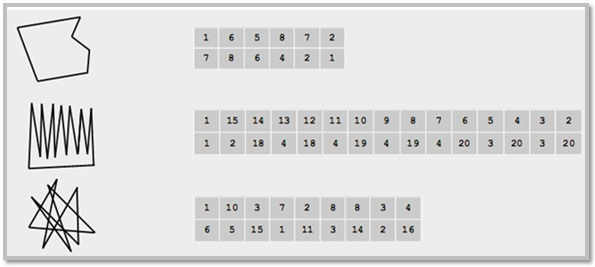
\includegraphics{2.jpg}
			\caption{سمت چپ، آنچه ما مي‌پنداريم و سمت راست، آنچه الگوريتم مي‌بيند.}
	\end{center}
   	\label{شکل 2}
\end{figure}  
\section*{نکاتی راجع‌به فاصله
\footnote{\lr{Distance}}}
	\addcontentsline{toc}{section}{نکاتی راجع‌به فاصله}
تعريف فضاي متريک: به مجموعه‌اي گفته مي‌شود که نوعي فاصله (متر) ميان اعضاي آن تعريف شده باشد. \\
مثال‌هاي فضاي متريک:
\begin{enumerate}
	\item 
	متر (فاصله) اقليدسي: يک خلبان هلي کوپتر فاصله ها به صورت متر اقليدسي مي‌سنجد.   
	$$d=\sqrt{ (x_{1}-x{0})^{2} + (y_{1}-y_{0})^{2} }$$
	   \begin{figure}[h!]
		\begin{center}
			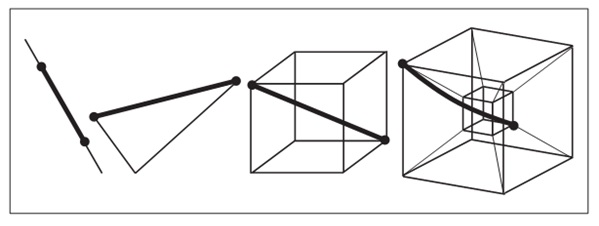
\includegraphics{3.jpg}
			\caption{فاصله اقليدسي در فضاي 1، 2، 3 و 4 بعدي}
		\end{center}
	   	\label{شکل 3}
	\end{figure}
\\
\\
\item 
متر 
\lr{Manhattan}
: خيابان‌هاي محله منهتن نيويورک بدين صورت آرايش يافته است. معمولا تاکسي‌هاي محله منهتن فاصله يک نقطه از نقطه ديگر را با متر منهتن مي‌سنجند.                                                                       
(در فضای $n$-بعدی) 
$$d(x-y)=\sum_{k=0}^{n} |xk - yk|$$
	   \begin{figure}[h!]
	\begin{center}
		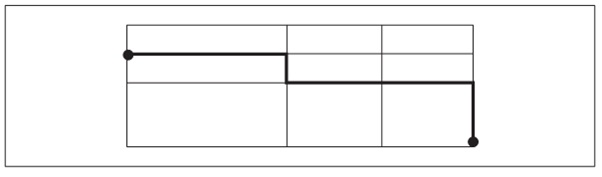
\includegraphics{4.jpg}
		\caption{\rl{متر منهتن}}
	\end{center}
   	\label{شکل 4}
\end{figure}
\item 
	متر (فاصله) ماکزيمم: عبارت است از مؤلفه ماکزيمم اختلاف دو نقطه:   
	$$d= Max{d(x,y)}$$ 
\end{enumerate}
\chapter{روش افزایشی
}

\section*{مقدمه}
	\addcontentsline{toc}{section}{مقدمه}
	اجازه دهيد قبل از ورود به مباحث جدي اين فصل، کار را با يک توضيح ساده که در عين حال مي تواند مفهوم آلگوريتم افزايشي را به خوبي منتقل نمايد شروع کنيم.\\
	
	فرض کنيد شخصي در حال ديدن يک فيلم پليسي است که قتلي در آن اتفاق افتاده است. بيننده از ابتدا که شروع به ديدن فيلم مي‌کند، يک فرضيه در ذهن دارد که چه کسي مرتکب قتلي شده که در ابتداي فيلم رخ داده و چگونه و چرا اين امر صورت گرفته است. در طول ديدن فيلم، هر نشانه‌ي جديد ممکن است فرضيه اول را تاييد يا تکميل کند و يا نياز باشد در آن تجديد نظر شود. همچنين ممکن است حتي رها شده و مجددا فرموله شود. تنها در پايان فيلم است که تمام سرنخ‌ها بدست مي‌آيند و بيننده راز جرم و جنايت را حل کرده است. البته با اين فرض که بيننده به اندازه کافي باهوش است و نويسنده فيلم نيز  داستان را صحيح و منصفانه تعريف کرده است. \\
	
	الگوريتم‌هاي افزايشي نيز چنين وضعيتي دارند. در بعضي موارد، الگوريتم تنها قادر به بيان و توضيح وضعيت فعلي به عنوان يک راه حل مسئله است. اگر چه ممکن است اين راه حل، مخالف پاسخ نهايي باشد. اين وضعيت مي‌تواند زماني اتفاق افتد که بخشي از ورودي‌ها خيلي ناقص است و يا يک وضعيت منسجم براي ورودي‌ها وجود ندارد. بنابراين حدس‌زدن پاسخ نهايي در طول حل مسئله، هميشه ما را به پاسخ نهايي رهنمون نمي‌کند.\\
	
	براي ساختن يک چند ضلعي با کمک تعدادي نقطه داده‌شده، تا زماني که تمام ورودي‌ها پردازش نشوند، مرز چندضلعي بدست نمي‌آيد. گاهي ممکن است با ورود تعدادي نقطه، ساده‌بودن چندضلعي به هم بخورد و تا زماني که همه ورودي پردازش نشده است، چند ضلعي مشخص نمي‌شود. همان‌طور که در مثال ديدن فيلم جنايي، فرضيه‌هاي بدست‌آمده در مراحل مختلف، ممکن است بارها با اشتباه روبرو شوند و يا سرنخ‌هاي اوليه و بينش‌هاي سازمان‌يافته نتوانند به فرآيند بدست‌آوردن پاسخ نهايي کمک کنند. در اين مثال نيز هرگونه حدسي براي جواب ممکن است غلط از کار درآيد. \\
	{مثال 1 \large}\\
	يک مثال ساده محاسباتي ديگر از روش افزايشي درجي، مي‌تواند پيداکردن کوچکترين عدد، در يک آرايه از اعداد صحيح باشد. در ابتدا اولين عدد را براي پاسخ مسئله کانديد مي‌نماييم و سپس جلو مي‌رويم. با هر عدد جديد از  آرايه، پاسخ قبلي را به روز مي‌کنيم و هرگاه به عددي کوچکتر برخورد کرديم، آن‌ را جايگزين پاسخ قبلي مي‌نماييم. کوچکترين عدد صحيح در ميان اعداد ديده‌شده، پاسخ مسئله تا کنون خواهد بود؛ بنابراين تا آخرين عدد، هر حدسي براي پاسخ مسئله ممکن است غلط باشد و پاسخ مسئله وقتي بدست مي‌آيد که تمام اعداد آرايه بررسي شده باشند.\\
	
	روش محاسباتي افزايشي ، يک روش محاسباتي نسبتا ساده است که در حل مسائل محاسباتي و از جمله هندسه محاسباتي متعددي بکار گرفته مي‌شود. اين روش محاسباتي ويژگي هاي زير را دارد:
	\begin{itemize}
		\item 
		روش افزايش درجي، يک روش مناسب براي حل مسائل محاسباتي و هندسه محاسباتي مي‌باشد.
		\item 
		براي حل يک مسئله با روش افزايشي ابتدا کار را با يک ورودي آغاز مي‌کنيم و در هر مرحله، ورودي مسئله را يکي افزايش مي‌دهيم.
		\item 
		در هر مرحله، با افزايش ورودي، پاسخ بدست آمده در مرحله قبلي را به‌روز مي‌کنيم.
		\item 
		در انتها، با اتمام ورودي‌ها، پاسخ مسئله نهايي به‌ دست مي‌آيد. 
		\item 
		در بعضي مسائل، تا انتها نمي‌توان پاسخ صحيح مسئله را ديد.
		\item 
		در طول الگوريتم، با بررسي داده‌ها در هر مرحله، پاسخ مسئله مرحله به مرحله ساخته مي‌شود. پاسخ مسئله تنها در انتهاي الگوريتم قابل رؤيت خواهد بود.
	\end{itemize}
با توجه به تعاريف و توضيحات داده‌شده، اکنون وقت آن رسيده است که به توضيح نمونه‌هايي از مسائلي که با اين روش حل مي‌شوند، بپردازيم. اولين مسئله، مرتب‌سازي درجي خواهد بود که يک مسئله ساده است. در حقيقت با توضيح اين مسئله که معمولا در درس ساختمان داده‌ها عنوان مي‌شود، مروري بر توضيحات بالا خواهيم داشت و پس از آن، به مسائل هندسي خواهيم پرداخت.
\section*{مرتب‌سازی درجی}
	\addcontentsline{toc}{section}{مرتب‌سازی درجی}
\textit{	فرض کنيد آرايه‌اي از اعداد حقيقي داده شده است. مي‌خواهيم داده‌هاي درون اين آرايه را مرتب نماييم.\\}
	
	مرتب‌سازي به روش درجي، ساده‌ترين نوع مرتب‌سازي است. يک مثال ساده و ملموس از مرتب‌سازي به روش درجي، مرتب‌كردن كارت‌هاي بازي مي‌باشد. براي مرتب‌كردن كارت‌ها  به روش درجي، ابتدا از اولين کارت شروع مي‌کنيم. در هر مرحله، يك كارت را خارج نموده و با كارت‌هايي که تا به‌ حال مرتب شده است، يکي يکي مقايسه مي‌کنيم. سپس كارت مذكور را منتقل نموده و در محل خود قرار مي‌دهيم. اين عمل را تا زماني که ديگر کارتي باقي نماند، و در همه جاي اصلي خود قرار گرفته باشند ادامه مي دهيم. \\
	فرض کنيد آرايه 
	$A[0,1,2,\dots,n-1]$
	 شامل $n$ عدد حقيقي داده شده است. مي خواهيم اعداد اين آرايه را مرتب نماييم.\\
	 شبه کد آلگوريتم درجي اين کار را انجام مي دهد:

\begin{LTR}
	\begin{Verbatim}[tabsize=0]
	insertion_Sort(A_n)
	for  i=2 to n   Do
	    key = A[i];
	    j = i - 1;
	    while   j > 0 && A[j] > key
	        A[j+1] = A[j]
	        j = j – 1;
	    A[j+1]= key;
	\end{Verbatim}
\end{LTR}
	نقطه قوت مرتب‌سازي درجي اين است كه نسبتاً ساده و قابل درک و اجراي آن آسان است. در مقابل، نقطه ضعف آن اين است كه براي مرتب‌کردن مجموعه‌اي بزرگ از داده‌ها مناسب نيست. چرا که براي رسيدن به پاسخ نهايي، بايد هر عدد را با  کليه داده‌ها مقايسه نماييم و اين، وقت نسبتا زيادي خواهد گرفت. \\
	مثال: مجموعه اعداد
	$"34 \hspace*{0.25cm} 8 \hspace*{0.25cm}  64 \hspace*{0.25cm}  51 \hspace*{0.25cm}  32 \hspace*{0.25cm} 21"$
	 داده شده است. مي خواهيم با روش مرتب سازي درجی که يک روش افزايشی است اين مجموعه را مرتب نماييم.
	 \begin{center}
	$$34 \hspace*{0.25cm} 8 \hspace*{0.25cm}  64 \hspace*{0.25cm}  51 \hspace*{0.25cm}  32 \hspace*{0.25cm} 21$$
		$$\textcolor{red}{34} \hspace*{0.25cm} 8 \hspace*{0.25cm}  64 \hspace*{0.25cm}  51 \hspace*{0.25cm}  32 \hspace*{0.25cm} 21$$
		$$\textcolor{red}{34 \hspace*{0.25cm} 8} \hspace*{0.25cm}  64 \hspace*{0.25cm}  51 \hspace*{0.25cm}  32 \hspace*{0.25cm} 21$$
			$$\textcolor{blue}{34 \hspace*{0.25cm} 8 \hspace*{0.25cm}}  \textcolor{red}{64} \hspace*{0.25cm}  51 \hspace*{0.25cm}  32 \hspace*{0.25cm} 21$$
				$$\textcolor{blue}{34 \hspace*{0.25cm} 8 \hspace*{0.25cm}  64 \hspace*{0.25cm}}  \textcolor{red}{51} \hspace*{0.25cm}  32 \hspace*{0.25cm} 21$$
						$$\textcolor{blue}{34 \hspace*{0.25cm} 8 \hspace*{0.25cm}  64 \hspace*{0.25cm}  51 \hspace*{0.25cm}}  \textcolor{red}{32} \hspace*{0.25cm} 21$$
										$$\textcolor{blue}{34 \hspace*{0.25cm} 8 \hspace*{0.25cm}  64 \hspace*{0.25cm}  51 \hspace*{0.25cm}  32 \hspace*{0.25cm}}
										\textcolor{red}{21} $$
$$\textcolor{blue}{34 \hspace*{0.25cm} 8 \hspace*{0.25cm}  64 \hspace*{0.25cm}  51 \hspace*{0.25cm}  32 \hspace*{0.25cm}
{21}} $$
	 \end{center}
	\subsection*{پيچيدگي زماني مرتب‌سازي درجي}
	بهترين حالت
	\footnote{\lr{Best Case}}
	 : بهترين حالت براي مرتب کردن اعداد به روش افزايشي ، حالتي است که اعداد از قبل مرتب باشند. در اين حالت هر عدد در محل صحيح خود قرار دارد و نيازي به مقايسه نيست. بنابراين پيچيدگي زماني مرتب سازي درجي $O(n)$ خواهد بود.\\
	 
	 بدترين حالت :  بدترين حالت براي مرتب کردن اعداد به روش افزايشي درجي، حالتي است که اعداد برعکس مرتب شده باشند، در اين حالت هر عدد بايد با کليه اعداد قبلي مقايسه و آنگاه در انتهاي آرايه قرار گيرد. در اين حالت پيچيدگي زماني مرتب سازي $O(n^2)$ خواهد بود.\\
	 
	 حالت متوسط: پيچيدگي زمان متوسط يک آلگوريتم براي شرايطي رخ مي دهد که عناصر به صورت تصادفي داده شوند. بنابراين حالت متوسط آلگوريتم مرتب سازي درجي در حالتيکه اعداد به صورت تصادفي پخش شده باشند محاسبه مي‌شود.  اگر به شبه کد بالا توجه نماييد در هر تکرار حلقه‌ي بيروني، حلقه‌ي داخلي براي يافتن محل مناسب درج عنصر جديد به طور ميانگين نصف ليست مرتب شده را پيمايش مي‌کند.به اين معني مطابق شبه کد بالا در هر تکرار حلقه‌ي بيروني، حلقه‌ي داخلي براي يافتن محل مناسب درج عنصر جديد به طور ميانگين نصف ليست مرتب شده را پيمايش مي‌کند. چرا که به طور متوسط نيمي از عناصر در $A[1\dots j]$
کم‌تر از $Key$  هستند و نيمي بزرگ‌تر از آن مي‌باشند. بنابراين در حالت ميانگين از مرتبه‌ي نصف تعداد ليست مرتب شده زمان مصرف مي شود. بنابراين:\\
	 $$T(n)= 1+ \frac{2}{2} + \frac{3}{2} + \dots + \frac{n-1}{2} = \frac{n(n-1)}{4} \approx \frac{n^{2}}{4} \in O(n^{2})$$
	    بنابراين ثابت مي شود که بطور متوسط، پيچيدگي زماني مرتب سازي درجي مشابه بدترين حال
	   $ \theta (n^{2})$
	    مي باشد. 
	    \section*{ساختن چندضلعي ستاره‌ شكل}
	 	\addcontentsline{toc}{section}{ساختن چندضلعي ستاره‌ شكل}
	 	فرض كنيد مجموعه نقاط
	 	$S = {s_{0}, \dots, s_{0}}$ 
	 	در صفحه داده شده است. چگونه مي‌توان با استفاده از مجموعه نقاط $S$ يك چندضلعي ستاره‌شكل 
	 	\footnote{\lr{Star-Shaped}}
	 	 ساخت؟\\
	 	با توضيحاتي که ارائه شد و مثال هايي که زده شد مقداري با روش افزايشي آشنا شديم. اکنون مي توانيم به مسائل هندسي و حل آن با کمک روش افزايشي بپردازيم.\\
	 	در اين بخش مي خواهيم به روش افزايشي با کمک مجموعه اي از نقاط داده شده يک چندضلعي ستاره شکل بدست آوريم. براي انجام اين کار مقدمات و تعاريف نسبتا زيادي لازم است که در زير خواهد آمد. \\
	 	\textbf{مقدمه و کاربرد: }
	 	در يک تعريف نسبتاً ساده، مي‌توان علم هندسه را علم انجام قواعد و دستورات بر روي نقطه، خط و چندضلعي دانست. قواعدي از قبيل دوري و نزديکي، داخل و خارج، شباهت و تفاوت و ... .\\
	 	در اين ميان، خط نقش و اهميت خاصي دارد. ترسيم خط راست بسيار ساده‌تر از منحني است و کاربردهاي آن در دنياي واقعي بي‌شمار است. در معماري بناهاي کلاسيک از خطوط راست استفاده مي‌شود. خيابان‌ها و اتوبان‌ها از خطوط راست تشکيل شده‌ اند. در تئوري فيزيک کلاسيک، نور از شعاع‌هاي راست تشکيل شده است. در تئوري ديد و رؤيت پذيري، پرتو ديد و شعاع اشعه‌هاي سنسورها از خطوط راست ايجاد شده اند.\\
	 	در هندسه قديم و هندسه مدرن، پاره‌خط کاربرد‌هايي بيش از خط دارد. پاره‌خط، خط راستي است که ابتدا و انتهاي آن با کمک دو نقطه محدود شده است. به عبارت ديگر، يک پاره‌خط، از دو طرف محدود مي‌باشد. با کمک پاره‌خط‌ها، چندضلعي‌ها ساخته مي‌شوند. بسياري از محاسبات مسائل هندسي، در مورد چندضلعي‌ها مي‌باشد. چندضلعي¬ها اشکال هندسي هستند که براي نمايش بسياري از اشياي موجود در دنياي واقعي به کار مي¬روند و اساس علم هندسه را تشکيل مي دهد. 
	 	\section*{هسته چندضلعی}
	 		 	\addcontentsline{toc}{section}{هسته چندضلعی}
	 	در اين بخش مي خواهيم به عنوان اولين کاربرد از روش افزايشي براي يافتن چندضلعي ستاده شکل استفاده کنيم. براي اين کار لازم است ابتدا تعريف هسته را بدانيم. به منظور آشنائي با اين مفهوم مي‌توانيد يک سالن بزرگ شامل تعدادي فروشگاه و بخش‌هاي اداري متعدد را در نظر بگيريد و يک مرکز اطلاعات که در قسمتي از آن وجود دارد. افراد براي کسب اطلاع به مرکز اطلاعات مراجعه مي‌کنند و پاسخ سؤالات خود را مي‌گيرند. در اينجا يک سؤال مطرح مي‌شود: "چه محلي در سالن، بهترين مکان براي اين مرکز اطلاعات مي‌باشد؟" بدون شک، بهترين مکان براي اين مرکز اطلاعات، محلي است که از تمام نقاط سالن و درهاي ورودي قابل رويت باشد تا افراد به سادگي بتوانند از هر نقطه و از هر فاصله‌اي، مرکز اطلاعات را ببينند و به آن مراجعه نمايند. با نگاهي متفاوت، بهترين موقعيت مکاني براي مرکز اطلاعات، موقعيتي است که از آنجا، هر شخصي که در مرکز اطلاعات حضور دارد، بتواند تمام فضاي فروشگاه را ببيند. به چنين مکاني در فروشگاه که از آن تمام نقاط قابل رؤيت باشد، هسته فروشگاه مي‌گويند. و اگر چنين مکاني در فروشگاه وجود داشته باشد فروشگاه ستاره شکل است.
	 	\begin{figure}[h]
	 		\begin{center}
	 			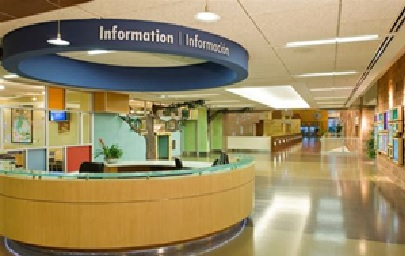
\includegraphics{5.jpg}
	 			\caption{یک مرکز اطلاعات}
	 		\end{center}
 		   	\label{شکل 5}
	 	\end{figure}
	 	نکات فوق بصورتي دقيق تر و با تعابير هندسي تعريف خواهد شد.\\
	 	
	 	دريک تعريف ابتدايي، چندضلعي ساده
	 	\footnote{\lr{Simple Polygon}}
	 	  $P$
	 	  ، ناحيه‌اي در صفحه است که توسط تعداد محدودي پاره‌خط متصل به هم احاطه شده است؛ به طوريکه اين مجموعه پاره‌خط‌ها، يک دور ساده ايجاد مي‌کنند. در يک چندضلعي ساده، دو پاره‌خط (ضلع) مجاور، تنها در نقاط پاياني خود (رئوس 
	 	  $P$
	 	  )
	 	  با يکديگر تقاطع دارند. و اشتراک پاره‌خط‌ها (اضلاع) غير مجاور تهي است. اگر چه بيان فوق مقداري مفهوم چندضلعي ساده را بيان مي کند ولي چندضلعي را به صورت دقيق‌تر و با کمک عبارات رياضي مي توان به شکل زير تعريف کرد.
	 	  \section*{تعریف چندضلعی}
	 	  	 		 	\addcontentsline{toc}{section}{تعریف چندضلعی}
	 	   يک چند¬ضلعي در صفحه، شکلي هندسي است که از يک مجموعه¬ي مرتب از نقاط در صفحه تشکيل شده است. فرض كنيد 
	 	   $V={v_{0}, \dots, v_{n-1}}$
	 	   ، مجموعه اي از $n$ نقطه در صفحه باشد. همچنين فرض كنيد:
	 	   $$e_{1}=v_{0}v_{1}, e_{2}=v_{1}v_{2}, \dots , e_{i}=v_{i-1}v_{i}, e_{n}=v_{n-1}v_{0},$$
	 	   $n$
	 	   پاره خط باشند كه نقاط را به هم متصل مي‌نمايند؛ آنگاه ناحيه محصورشده توسط مجموعه 
	 	   $C= {e_{1},e_{2},... ,e_{n} }$
	 	    تشكيل يك چندضلعي ساده مي‌دهد؛ اگر و تنها اگر شرايط زير برقرار باشند.
	 	    \begin{enumerate}
	 	    	\item 
	 	    	محل تلاقي هر جفت پاره‌خط مجاور، تنها نقطه مشترك آن‌ها باشد.
	 	    	$$\forall i \in {1,2,\dots ,n-1}  		e_{i} \bigcap e_{i+1} = v_{i} $$
	 	    	\item 
	 	    	هيچ دو پاره‌خط غيرمجاور يكديگر را قطع نكنند.
	 	    	$$\forall j \in {1,\dots ,n-1} j\neq i+1 , i-1 \rightarrow   e_{i} \bigcap e_{j} = \varnothing $$
	 	    \end{enumerate}
 	    شرط اول تضمين مي‌کند که مرز چندضلعي بسته باشد. به عبارت ديگر، انتهاي هر ضلع به ابتداي ضلع بعدي متصل شده باشد. شرط دوم نيز تضمين مي‌کند که بين هيچ دو ضلع غير مجاور، تقاطع وجود نداشته باشد. بدين ترتيب چنانچه دو شرط فوق برقرار باشد، يک چندضلعي ساده ايجاد مي¬شود که پاره¬خط¬هاي سازنده‍ي آن را اضلاع 
 	    \footnote{\lr{Edge}}
 	     چندضلعي و نقاط سازنده¬ي آن را رئوس 
 	      	    \footnote{\lr{Vertex}}
 	      چندضلعي مي¬نامند. چنانچه از دو شرط فوق، شرط دوم برقرار نباشد، چندضلعي تشکيل¬شده يک چندضلعي غير¬ساده مي¬باشد. مسائل هندسه¬ي محاسباتي اغلب بر چند¬ضلعي¬¬هاي ساده تمرکز مي¬کنند. در نتيجه ما نيز اين رويکرد را دنبال مي‍کنيم. شکل زير را ملاحظه نماييد.
 	      	 	\begin{figure}[h]
 	      	\begin{center}
 	      		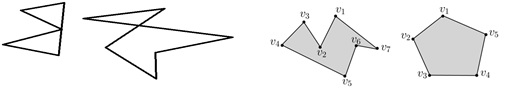
\includegraphics{6.jpg}
 	      		\caption{شکل سمت چپ، دسته¬بندي چندضلعي¬ها به چندضلعي¬هاي ساده و غير ساده. شکل سمت راست:  دسته بندي چندضلعي ها به چندضلعي محدب و غير محدب }
 	      	\end{center}
       	   	\label{شکل 6}
 	      \end{figure}
       چنانچه پاره‌خط اول و پاره‌خط انتهايي اشتراکي نداشته باشند، يک زنجير باز 
        	      	    \footnote{\lr{Open Chain}}
        	      	     خواهيم داشت. در حقيقت زنجير باز به صورت زير تعريف مي‌شود.\\
        	      	    فرض کنید 
         $$e_{1}=v_{0}v_{1},\hspace{0.125cm} e_{2}=v_{1}v_{2}, \dots , \hspace{0.125cm} e_{i}=v_{i-1}v_{i}, \hspace{0.125cm} e_{n-1}=v_{n-1}v_{0}$$
         $n-1$
         پاره‌خط باشند و شرایط زیر برقرار باشند.
         $$\forall i \in {1,2, \dots, n-2} \hspace{0.5cm} e_{i} \bigcap e_{i+1} = v_{i}$$
    	$$\forall j \in {1,\dots ,n-1} \hspace{0.5cm} j\neq i+1 , i-1 \hspace{0.25cm} \rightarrow \hspace{0.25cm}  e_{i} \bigcap e_{j} =\varnothing $$         
          با استفاده از  قضيه خم جردن، مي‌توان گفت چندضلعي ساده، صفحه را به دو ناحيه تقسيم مي¬کند: ناحيه¬ي کران¬دار
                  	      	    \footnote{\lr{Bounded}}
            که داخل چندضلعي قرار دارد و ناحيه¬ي بي‌کران 
                    	      	    \footnote{\lr{Unbounded}}
             که بيرون چندضلعي واقع شده است. معمولاً در مسائل هندسه‍ي محاسباتي، مرز  
                     	      	    \footnote{\lr{Boundary}}
             چندضلعي نيز جزء ناحيه¬ي داخل چندضلعي محسوب مي¬شود. به عبارت ديگر، بر خلاف آنچه در هندسه دبيرستاني مي دادند، يک چندضلعي در هندسه محاسباتي تنها يک مرز نيست؛ بلکه چندضلعي شامل مرز و ناحيه‌ي کران‌دار محدود شده توسط مرز مي‌باشد. \\
             
             در يک دسته¬بندي مي¬توان چندضلعي¬هاي ساده را به دو دسته¬ي چندضلعي¬هاي محدب 
                                  	      	    \footnote{\lr{Convex}}
              و چندضلعي¬هاي غيرمحدب
                                   	      	    \footnote{\lr{Non-Convex}}
                طبقه‌بندي کرد. اگر چه در اين مورد بطور مفصل در بخش هاي بعدي صحبت خواهد شد. جهت آشنائي ابتدائي مي توان گفت  چند¬ضلعي ساده¬ي $P$ يک چندضلعي محدب است؛ اگر و تنها اگر هر پاره¬خطي که دو نقطه¬ي دلخواه از داخل $P$ را به هم وصل مي-کند، کاملاً داخل $P$ قرار گيرد. در غير اين صورت $P$ يک چندضلعي نامحدب است. از نگاهي ديگر، در چندضلعي محدب $P$، همه¬ي زواياي داخلي چندضلعي کوچکتر از $\pi$ راديان مي¬باشند؛ در حالي که در يک چندضلعي نامحدب، حداقل يک زاويه¬ي داخلي بزرگتر از $\pi$ راديان وجود دارد. شکل 2 را ملاحظه کنيد.\\

                اکنون که تعريف چندضلعي را بيان کرديم، به عنوان پيش‌نياز به يک موضوع ديگر نياز داريم و آن رؤيت پذيري است. اگر چه اين موضوع خود آنقدر بزرگ و گسترده و پرکاربرد است که به بزرگترين و جذاب ترين موضوع در هندسه محاسباتي تبديل شده است. ولي ما در اينجا به چند تعريف و نکته ابتدائي آن فقط در حد مورد نياز اشاره مي کنيم. ولي در فصول آينده مجددا به آن اشاره خواهيم داشت.
                \section*{رویت پذیری}
                	 		 	\addcontentsline{toc}{section}{رویت پذیری}
                در هندسه "ديدن" و "رويت پذيري" از يک تعريف بسيار ساده آغاز و سپس به يکي از مباحث مهم و پيچيده با کاربردهاي فراوان در هندسه محاسباتي- که هم اکنون نيز به عنوان يک زمينه علمي جذاب با مسائل باز بسيار مطرح است- تبديل مي‌شود.\\
                
                يک نمونه از کاربردهاي رويت‌پذيري، بهينه‌سازي حرکت ربات‌هاي جستجوگر است که يک هدف ثابت يا متحرک را دنبال مي‌کنند. در مسئله فوق، در يک فضاي بسته که با يک چندضلعي شبيه‌سازي مي‌شود  تعدادي ربات‌ با داشتن قابليت ديد، از برخورد با موانع پرهيز و به هدف دسترسي پيدا مي‌کنند. در اين مسئله، رؤيت‌پذيري در هدايت ربات‌ها کاربرد پيدا مي‌کند.\\
                مسئله مسير‌يابي در سيستم‌هاي اطلاعات جغرافيايي که با يک شبکه گراف شبيه‌سازي مي‌شود نمونه ديگري از کاربرد‌هاي رويت‌پذيري مي‌باشد. در اين مسئله، مسيريابي يک متحرک با کمک رويت‌پذيري صورت مي‌گيرد.\\
                رويت‌پذيري در هندسه معماري نيز کاربرد دارد. طراحي پلان و ابعاد يک ساختمان، چشم انداز، جهت و نماي ساختمان و تقسيم‌بندي بخش‌هاي درون يک ساختمان با کمک رويت پذيري صورت مي‌گيرد. در حقيقت رؤيت پذيري در طراحي ديد و چشم انداز مناسب و افزايش  بهره گيري از نور، تناسب بخش‌هاي مختلف داخلي نقش دارد. \\
                مسئله رؤيت‌پذيري در طراحي و جانمايي شبکه سنسور و طراحي سيستم امنيت براي ساختمان‌ها و نيز نورپردازي سالن‌ها و نماي ساختمان‌ها کاربرد دارد.\\
                يک کاربرد رايج ديگر مسئله رؤيت‌پذيري، امنيت و حفاظت از يک محيط توسط نگهبانان و يا دوربين‌هاي مدار بسته مي‌باشد. \\
                مسئله‌ي معروف نگارخانه‌ي هنر و تلاش براي کاهش تعداد نگهباناني که از نگارخانه مراقبت مي‌کنند،  يکي از معروف‌ترين کاربردهاي رويت‌پذيري مي‌باشد. در بخش بعدي به اين مسئله خواهيم پرداخت. ادامه اين بخش ما را از مسيرمان مقداري دور مي کند و لي با توجه به تعريف رؤيت پذيري ديدن صورت مسئله نگارخانه هنر در اينجا خالي از لطف نيست. اگر چه بعدها به اين مسئله بيشتر خواهيم پرداخت. اين کار ما را مقداري از مسيرمان منحرف مي کند ولي با توجه به تعريف رؤيت پذيري ديدن صورت مسئله گالري هنر در اينجا خالي از لطف نيست. اگر چه بعدها به اين مسئله بيشتر خواهيم پرداخت.\\
                \section*{نگارخانه هنر}
             	\addcontentsline{toc}{section}{نگارخانه هنر}
                فرض کنيد يک نگارخانه با سالن‌ها و راهروهاي پيچ در پيچ وجود دارد که محل نگهداري تابلوها و آثار هنري گران‌قيمت است. به دليل اهميت و ارزش آثار هنري، نگارخانه بايد به طور دائم و کامل توسط نگهبانان يا دوربين‌هاي مداربسته تحت کنترل قرار گيرد. همچنين نکات زير در مورد نگارخانه و نگهبانان آن مطرح است:\\
                دوربين‌ها بايد به نحوي در مکان‌هاي مختلف نگارخانه نصب شوند که تعدادشان کمينه شود؛ بدين وسيله، در هزينه‌هاي مراقبت از نگارخانه صرفه‌جويي مي‌شود. در عين حال، بايد تمام نقاط مراقبت شوند. بنابراين نبايد تعداد دوربين‌ها به اندازه‌اي کم باشد که بخش‌هايي از نگارخانه توسط آن‌ها پوشش داده نشود. علاوه بر آن، هرچه تصاوير ارسالي از دوربين‌ها کمتر باشد، نظارت و کنترل آن‌ها راحت‌تر خواهد بود. در واقع در بعضي مسائل، کاهش هم پوشاني دوربين‌ها اهميت دارد.\\
                براي بررسي و تحليل مسئله نگارخانه هنر، مي‌توان نگارخانه را توسط يک چندضلعي با n رأس و دوربين‌ها را با نقاط مدل کرد. \\
                مسئله‌ي نگارخانه هنر ابتدا در سال 1973 توسط کلي  
                \footnote{\lr{Klee}}
                مطرح شد. او سؤال زير را مطرح کرد:\\
       "چه تعداد نگهبان براي کنترل و حفاظت از يک نگارخانه مورد نياز است؟"\\
       در مسئله کلاسيک نگارخانه هنر، شرايط زير در نظر گرفته مي شود: 
       \begin{itemize}
       	\item 
       		نگارخانه يک n ضلعي ساده مي باشد.  
\item 
       	هر نگهبان به عنوان يک نقطه‌ي ثابت در نظر گرفته مي‌شود که قادر است تمامي جهات را ببيند و داراي دامنه‌ي ديد 360 درجه و با شعاع ديد بي‌نهايت مي‌باشد.
       	\item 
       	نگهبان‌ها نمي‌توانند پشت ديوارها را ببينند.
       \end{itemize}
   مسائل جذاب، ارزشمند و در عين حال کاربردي در زمينه نگارخانه هنر وجود دارد که بعضي شرايط فوق را ناديده مي‌گيرند. به عنوان مثال، نگارخانه مي‌تواند ساده نباشد، بلکه تعدادي ستون در ميانه سالن‌ها و راهروها وجود داشته باشد. در اين حالت چندضلعي ساده نخواهد بود؛ حالت ديگر آن است که دامنه ديد نگهبان‌ها از 360 درجه کمتر باشد؛ در اين صورت اصطلاحا به آن آلفا گارد 
   \footnote{\lr{$\alpha$-Gard}}
    گويند. در حالتي ديگر، مي‌توان در نظر گرفت که شعاع ديد نگهبان‌ها محدود باشد و يا اينکه بجاي نگهبان، لامپ در نظر بگيريم و محل لامپ‌ها را در خارج نگارخانه قرار دهيم. در اين حالت مسئله نگارخانه هنر را مي‌توان به صورت زير نيز مطرح کرد:\\
    "براي روشنايي کامل ديوارهاي يک ساختمان، براي مثال يک زندان، چه تعداد لامپ مورد نياز است؟"\\
     در مورد هرکدام از زير مسائل فوق کارهاي تحقيقاتي بسياري شده است و مسائل باز متنوعي وجود دارد که نظر پژوهشگران را به خود جلب مي کند.\\
     براي مدل‌کردن مسئله کلي به تعاريف زير نياز داريم.\\
     \textbf{قابلیت دید
     \footnote{\lr{Visibility}}}
 :
به فرض  $x$ و $y$ دو نقطه درون چند ضلعي $P$ باشند. گوييم نقطه $x$ مي‌تواند نقطه $y$ را ببيند - يا $y$ قابل رؤيت براي $x$ است اگر 
$\overline{xy} \subseteq P$
باشد.
$$x \hspace{0.125cm} can \hspace{0.125cm} see \hspace{0.125cm} y \hspace{0.125cm} iff  \hspace{0.125cm} \overline{xy} \subseteq P$$
به عبارت ديگر، پاره‌خطي که دو نقطه $x$ و $y$ را به هم متصل مي‌کند، بطورکامل درون چندضلعي $P$ قرار گيرد. 
توجه : عبارت بالا نشان مي‌دهد $xy$ مي‌تواند با يك راس يا ضلع از چندضلعي $P$ تماس داشته باشد. به عبارت ديگر $xy$ مي‌تواند با مرز چندضلعي تماس داشته باشد.  \\
\begin{figure}[h!]
	\begin{center}
		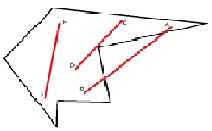
\includegraphics{7.jpg}
		\caption{
			:  نقطه $A$ براي نقطه $B$ قابل رؤيت نيست يعني نقاط $A$ و $B$  نمي‌توانند يکديگر را  ببينند. نقطه $C$ براي $D$ قابل رؤيت است. نقطه $E$ براي نقطه $F$ به وضوح قابل رؤيت است.}
	\end{center}
   	\label{شکل 7}
 	      \end{figure}
            \textbf{قابلیت دید واضح}
:  گوئيم دو نقطه $x$ و $y$ يکديگر را  به‌‌وضوح مي‌بينند يا براي يکديگر به وضوح قابل رؤيت
\footnote{\lr{Clear Visibility}}
 : هستند؛ اگر:
 $xy \subseteq P , xy \bigcap \partial P \subseteq {x,y}$
 بنابراين در حالتي که $y$ به‌‌وضوح براي  $x$ قابل رؤيت است، $xy$  نمي‌تواند با مرز چندضلعي تماس داشته باشد. 
 \begin{figure}[h!]
 	\begin{center}
 		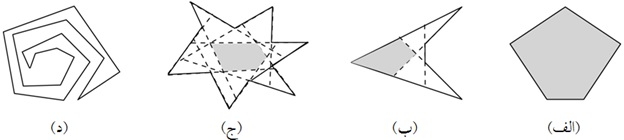
\includegraphics{8.jpg}
 		\caption{
هسته در چندضلعي‌هاي مختلف به رنگ تيره نشان داده شده است. (الف) هسته در يک چندضلعي محدب. (ب) هسته در يک چندضلعي پروانه‌اي شکل. (ج) هسته در يک چندضلعي ستاره‌اي شکل که پروانه‌اي شکل نمي‌باشد. (د) يک چندضلعي غير ستاره‌اي شکل که هسته آن تهي است.}
 	\end{center}
    	\label{شکل 8}
 \end{figure}
\\
            \textbf{هسته}
: هسته 
\footnote{\lr{Kernel}}
 يك چندضلعي  $P$ عبارت است از مجموعه كليه نقاطي از $P$ كه تمام چندضلعي را مي‌بينند.
$$kernel(P)={x\in P|x \hspace{0.125cm} can \hspace{0.125cm} see \hspace{0.125cm} y,\forall y\in P}$$
واضح است که وجود و بزرگي هسته‌ يک چندضلعي، بستگي به شکل آن دارد. ممکن است هسته يک چندضلعي تهي باشد و يا با خود چندضلعي برابر باشد. \\
            \textbf{چندضلعي ستاره‌شكل:}
 يك چندضلعي را ستاره‌شكل 
 \footnote{\lr{Star-Shaped Polygon}}
  گوييم اگر هسته آن ناتهي باشد.\\
  \textbf{چندضلعي پروانه‌اي‌ شکل: }
  يك چندضلعي را پروانه‌اي شكل 
   \footnote{\lr{Fan-Shaped}}
   گوييم؛ اگر هسته آن شامل حداقل يكي از رأس‌هاي آن باشد.
  از آنجا که تمام نقاط يک چندضلعي محدب مي‌توانند يکديگر را ببينند، هسته يک چندضلعي محدب با خود آن برابر است.\\
  اکنون که مقدمات لازم براي بررسي مسئله ساختن چندضلعي ستاره شکل را مطرح کرديم، مجددا به عنوان يادآوري صورت مسئله را مجددا ذکر مي کنيم. \\
  فرض كنيد مجموعه نقاط 
    $S=\{s_{0}, s_{1},\dots ,s_{n-1}\} $
  در صفحه داده شده است. چگونه مي‌توان با استفاده از مجموعه نقاط $S$  يك چندضلعي ستاره‌شكل 
  \footnote{\lr{Star-Shaped}}
   ساخت؟\\
  همانطور که در توضيح روش افزايشي اشاره شد، ساختن پاسخ مسئله را ابتدا  با يک ورودي آغاز مي‌کنيم و در هر مرحله، ورودي مسئله را يکي افزايش داده، پاسخ قبلي را بهبود بخشيده و آن را به‌روز مي‌نماييم. 
 \begin{figure}[h!]
	\begin{center}
		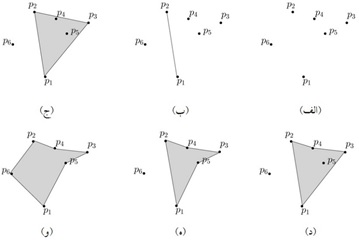
\includegraphics{9.jpg}
		\caption{
	اجراي الگوريتم چندضلعي ستاره‌اي شکل براي مجموعه‌اي از نقاط}
	\end{center}
   	\label{شکل 9}
\end{figure}  
  
  براي محاسبه يك چندضلعي ستاره‌شكل با کمک مجموعه نقاط 
  $S=\{s_{0}, s_{1},\dots ,s_{n-1}\} $
  	ابتدا با سه نقطه يک مثلث تشکيل مي‌دهيم و به دنبال آن مراحل ساخت يک چند چندضلعي ستاره‌شکل را دنبال مي‌کنيم. در هر مرحله نقطه جديد را به گونه‌اي به چندضلعي که تا کنون ساخته شده است، اضافه مي‌کنيم كه چندضلعي جديد ستاره‌شكل باقي بماند.  
  	اين مسئله يک پاسخ منحصر به فرد ندارد؛ بلکه پاسخ‌هاي متعددي براي مسئله مي‌تواند وجود داشته باشد. با کمک آلگوريتمي که در زير ارائه شده است، نوع خاصي چندضلعي ستاره‌اي بدست مي‌آيد كه هسته آن، شامل يکي از نقاط مجموعه $S$  يعني $s_{0}$ است.
\subsection*{الگوريتم افزايشي براي يافتن هسته چند‌ضلعی ستاره شکل}
الگوريتم افزايشي براي يافتن هسته چندضلعي ستاره شکل براي ساختن يک چندضلعي ستاره‌شکل به گونه اي عمل مي کند که  اولين نقطه ورودي همواه يکي از رؤس پاسخ نهايي خواهد بود.\\
مراحل آلگوريتم به صورت زير است.
\begin{itemize}
	\item 
		ابتدا با نقطه $s=s_{0}$ شروع مي‌کنيم.
\item 
	سپس با کمک نقاط ورودي دوم و سوم، يک مثلث مي‌سازيم که ستاره‌اي شکل است و شامل نقطه $s_{0}$ نيز مي‌باشد. 
	\item 
		فرض کنيد تا نقطه $i$ ام اضافه و با کمک اين نقاط تا کنون چندضلعي ستاره‌شکل ساخته شده است. اکنون در مرحله i ام هستيم و نقطه $i$ ام وارد شده است. نقطه $s_{i}$ به گونه‌اي به چندضلعي که تا کنون ساخته شده است، اضافه مي‌شود كه چندضلعي جديد ستاره‌شكل باقي بماند. براي اين کار، مرز چندضلعي موجود را از $s_{1}$ بصورت پادساعت‌گرد حول $s_{0}$  دور مي‌زنيم تا به رأسي مانند $s_{j}$ برسيم كه زاويه پادساعت‌گرد نقطه $s_{i}$ نسبت به $s_{0}$  و خط افق بلافاصله کمتر از $s_{j}$ نسبت به $s_{0}$ و خط افق باشد. در اين صورت $s_{i}$ قبل از $s_{j}$ قرار خواهد گرفت. \\
	در صورتي كه دور به پايان رسيد و چنين رأسي يافت نشد، در اين حالت زوايه پادساعت‌گردِ رأس جديد از همه بزرگتر خواهد بود. در اين حالت $s_{i}$ قبل از $s_{0}$ قرار خواهد گرفت.
	\item 
		با روش بالا نقاط بصورت پادساعت‌گرد با توجه به زاويه‌شان نسبت به $s_{0}$ به ترتيب به چندضلعي اضافه مي‌شوند. به عبارت ديگر $s_{p}$ قبل از $s_{q}$ قرار مي‌گيرد؛ اگر زاويه پادساعت‌گردش نسبت به $s_{0}$ و خط کوچکتر از $s_{q}$ باشد.
\end{itemize}
\textbf{روش مقایسه:}
روش مقايسه: به نظر مي رسد لازم باشد در مورد مقايسه موقعيت نقاط و تعيين محل نقطه جديد‌الورود که در حقيقت نکته اصلي آلگوريتم است و موجب مي‌شود چندضلعي ستاره شکل باقي بماند توضيح بيشتري داده شود. اولاً وقتي مي گوييم زاويه نقطه جديدالورود $s_{i}$ منظور زاويه پادساعت گردي است که 
$s_{i}s_{0}$
 با خط افق که از $s_{0}$ گذشته است مي سازد و آنرا با 
 $ \theta_{si}$
  نشان مي‌دهيم. وقتي براي انجام مراحل آلگوريتم افزايشي و اضافه‌کردن نقطه جديد
   $s_{i}$
  مرز چندضلعي موجود را بصورت پادساعت‌گرد دور مي‌زنيم و رئوس را يکي يکي با راس جديد 
  $s_{i}$
   مقايسه مي‌کنيم تا به رأسي مانند $s_{j}$ برسيم كه زاويه پادساعت‌گرد نقطه $s_{i}$ بلافاصله کمتر از زاويه $s_{j}$ است. روش مقايسه دو نقطه بدين صورت است که:
   \begin{center}
   	گوئیم نقطه
   	$s_{p}=(r_{p},\theta_{p})$
   	کوچکتر از نقطه
   		$s_{q}=(r_{q},\theta_{q})$
   		است و به صورت \\
   		$s_{p}<s_{q}$
   		نشان می‌دهیم اگر : 
   		$\theta_{q}>\theta_{p}$
   		یا
   		   		$\theta_{q}=\theta_{p}$
   		   		و
   		   		$r_{q}>r_{p}$
   		   		\\
   		   		   \end{center}
   		   		با اين روش، نقاط روي محيط چندضلعي به‌ صورت پادساعت‌گرد، به ترتيب زاويه از کوچک به بزرگ مرتب مي‌شوند. \\
   		   		
   		   		فرض کنيد در مرحله  $i$ام چندضلعي ستاره‌شكل به صورت
  $\{s_{0}, s_{1},\dots ,s_{i-1}\} $
   		   		   باشد که رئوس به ترتيب پادساعت‌گرد مرتب شده اند. وقتي نقطه 
   		   		   $s_{i}$
   		   		    اضافه مي‌شود، با ديگر رئوس مقايسه مي‌شود؛ اگر 
   		   		    $s_{j}$
   		   		     اولين نقطه‌اي در ترتيب پادساعتگرد باشد كه زاويه آن بلافاصله بزرگتر از 
   		   		     $s_{i}$
   		   		      است، چندضلعي ستاره‌شكل  به صورت 
   		$s_{0}, s_{1},\dots , s_{j-1}, s_{i}, s_{j}, \dots, s_{i-1}$
   		   		       در مي‌آيد. اگر چنين $s_{j}$ اي وجود نداشت، $s_{i}$ به آخر ليست اضافه مي‌شود. در اين صورت چندضلعي ستاره‌شكل  به صورت  
   		$s_{0}, s_{1},\dots ,s_{i-1}, s_{i}$
   		   		       در مي‌آيد.

 \begin{figure}[h!]
	\begin{center}
		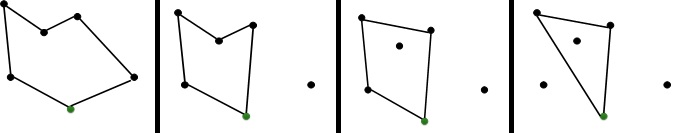
\includegraphics{10.jpg}
		\caption{
		اجراي مراحل الگوريتم ساخت چندضلعي ستاره‌اي شکل}
	\end{center}
   	\label{شکل 10}
\end{figure}  
\textbf{صحت الگوريتم}\\
اثبات: مراحل ساختن چندضلعي ستاره‌شكل با روش افزايشي بر روي نقاط اضافه‌شده صورت مي‌گيرد. در هر مرحله، نقطه جديد به رئوس قبلي چندضلعي اضافه مي‌شود. نحوه افزودن نقطه جديد به نقاط پوش چندضلعي، به صورت پرتو مي‌باشد. نقاط جديد به گونه‌اي به نقاط پوش اضافه مي‌شوند و اطراف هسته قرار مي‌گيرند؛ که به راحتي مي‌شود ثابت کرد همواره حداقل 
$s_{0}$
 تمام رئوس از جمله رأس جديد $s_{i}$ را مي‌بيند.\\
 
     \textbf{آنالیز الگوریتم}\\
يافتن چندضلعي ستاره‌شكل با کمک الگوريتم افزايشي درجي همانند مرتب‌سازي درجي مي‌باشد. تمام نقاط يکي يکي در محل مناسب به نقاط قبلي پوش محدب اضافه مي‌شوند. انتخاب محلي مناسب براي نقطه جديد با مقايسه زاويه پادساعت‌گرد آن نقطه نسبت به $s_{0}$ با نقاط قبلي چندضلعي ساخته‌شده صورت مي‌گيرد. اين مقايسه در مرحله $i$ام داراي پيچيدگي برابر $O(i)$ خواهد بود؛ بنابراين زمان کلي آلگوريتم برابر خواهد بود با:\\
$$T(n)= \sum_{i}^{}O(i)=O(n^{2})$$
\section*{تمرین}
\addcontentsline{toc}{section}{تمرین}
مسئله 1 (ساده): نشان دهيد رويت‌پذيري داراي خاصيت تقارن  
\footnote{\lr{Symmetry}}
است. بدين معني که اگر نقطه‌ي $p$ براي نقطه‌ي $q$ قابل رؤيت باشد، آن‌گاه نقطه‌ي $q$ نيز براي نقطه‌ي $p$ قابل رويت است.\\

مسئله2 (ساده): نشان دهيد رويت‌پذيري داراي خاصيت تعدي  نمي‌باشد. بدين معني که اگر نقطه‌ي $p$ نقطه‌ي $q$ و نقطه‌ي $q$ نقطه‌ي $r$ را در $p$ رويت کند، لزوما نقطه‌ي $p$ نقطه‌ي $r$ را رويت نمي‌کند. شکل 6 را ملاحظه نماييد. \\
\begin{figure}[h!]
	\begin{center}
		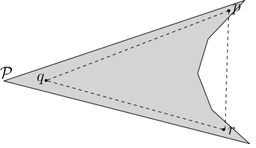
\includegraphics{11.jpg}
		\caption{رويت‌پذيري خاصيت تعدي ندارد.}
	\end{center}
   	\label{شکل 11}
\end{figure}  

مسئله3 : اثبات و يا رد کنيد: براي رؤيت‌پذيري چند ضلعي $P$ كافي است   $\partial P$ قابل رويت باشد.\\

اگر پاسخ شما به سوال منفي است، چندضلعي $P$ و يک مجموعه از نگهبان‌ها را طوري بسازيد که همه‌ي مرز چندضلعي قابل رويت باشد؛ ولي حداقل يکي از نقاط دروني آن با هيچ نگهباني رويت نشود. در غير اين صورت اگر پاسخ‌ شما مثبت است، بايد آن را ثابت کنيد.\\

مسئله 4: (اثبات و يا رد کنيد) براي رؤيت‌پذيري چندضلعي $P$  كافي است درون $P$  قابل رويت باشد.\\

مسئله 5: (اثبات و يا رد کنيد)  براي رؤيت‌پذيري چندضلعي $P$  كافي است رئوس $P$ قابل رويت باشد.\\

مسئله6: (اثبات و يا رد کنيد) هسته يک چندضلعي کراندار، درون چندضلعي و همبند است.\\

مسئله7 (مسئله سخت) آلگوريتمي ارائه دهيد که هسته يک چند ضلعي را به گونه‌اي محاسبه نمايد که مساحت آن بيشينه باشد. (بدست آوردن هسته بيشينه)\\

مسئله8: فرض کنيد مي‌خواهيم يک چندضلعي ستاره‌شکل را با کمک نقاط داده شده بسازيم. در دو حالت براي مسئله آلگوريتمي با زمان بهيته ارائه دهيد: حالت اول، زماني که نقاط برخط
\footnote{\lr{Online}}
  داده مي‌شود و حالت دوم، زماني که نقاط همگي از قبل داده شده اند.\\
  
مسئله 9: (مسئله سخت) آلگوريتمي  ارائه دهيد که هسته يک چندضلعي را در حالتي که شعاع ديد بي‌نهايت نيست، بلکه به ميزان $d$ مي‌باشد، محاسبه نمايد.( هسته با شعاع ديد محدود)\\

مسئله 10: (مسئله سخت)آلگوريتمي ارائه دهيد که هسته يک چندضلعي را در حالتي که زاويه ديد به جاي $2\pi$ مقدار $\pi$ است محاسبه نمايد. (هسته با زاويه ديد محدود)
\section*{پوش محدب}
\addcontentsline{toc}{section}{پوش محدب}
دومين مسئله هندسي که با روش افزايشي حل مي کنيم مسئله يافتن معروف پوش محدب مجموعه اي از نقاط داده شده مي باشد.\\
فرض کنيد مجموعه 
$P=\{P_{0},\dots ,P_{n} \}$
 شامل $n$ نقطه در صفحه داده شده است. همچنين فرض کنيد هيچ سه نقطه‌اي در يک امتداد نيستند. مي خواهيم  پوش محدب $P$ با استفاده از روش افزايشي.
\subsection*{مقدمه و کاربرد:}
 يافتن پوش محدب مجموعه اي از  نقاط داده شده با روش‌هاي متفاوتي امکان پذير است، که يکي از ساده ترين آنها روش افزايشي مي‌باشد.در اين روش يافتن، پوش محدب بطور طبيعي با افزودن يک به يک نقاط صورت مي‌پذيرد. همچون مسئله قبل ابتدا به تعاريف و مقدمات لازم پرداخته مي شود و سپس مسئله پوش محدب را تعريف و با روش افزايشي حل مي کنيم.\\
 در يک دسته¬بندي اوليه مي¬توان چندضلعي¬هاي ساده را به دو دسته¬ي چندضلعي¬هاي محدب  
 \footnote{\lr{Convex}}
 و چندضلعي‌هاي غيرمحدب  
 \footnote{\lr{Non-Convex}}
 دسته بندي کرد. چندضلعي‌هاي محدب و اساسا مسئله تحدب و پوش محدب در رياضيات و به خصوص هندسه، به دليل کاربردهاي گسترده‌اي که دارد، بسيار مورد توجه است. \\
 براي يک مجموعه محدب تعاريف متعددي وجود دارد و در مورد روش ساختن پوش محدب مجموعه‌اي از نقاط و يا پوش محدب يک چندضلعي، شيوه‌هاي مختلفي ارائه شده است.  در اين بخش، ابتدا پوش محدب را تعريف مي‌کنيم و سپس آلگوريتم يافتن پوش محدب براي مجموعه‌اي از نقاط با روش افزايشي درجي را توضيح مي‌دهيم. به دليل اهميت و کاربردهاي پوش محدب، در فصل‌هاي آينده اين مسئله با روش‌هاي متعددي حل خواهد شد. در ادامه اين فصل، پوش محدب مجموعه‌اي از نقاط به روش افزايشي مطرح خواهد شد. اگر چه در فصول بعدي، روش‌هاي ديگر که بعضا سريع‌تر هم هستند، براي ساختن پوش محدب ارائه مي‌شود، لاکن الگوريتم افزايشي پوش محدب، هم بسيار زيبا و هم بسيار الهام‌بخش است. ابتدا به تعريف پوش محدب مجموعه‌اي براي يک مجموعه محدب تعاريف متعددي وجود دارد و در مورد روش ساختن پوش محدب مجموعه‌اي از نقاط و يا پوش محدب يک چندضلعي، شيوه‌هاي مختلفي ارائه شده است.  در اين بخش، ابتدا پوش محدب را تعريف مي‌کنيم و سپس آلگوريتم يافتن پوش محدب براي مجموعه‌اي از نقاط با روش افزايشي درجي را توضيح مي‌دهيم. به دليل اهميت و کاربردهاي پوش محدب، در فصل‌هاي آينده اين مسئله با روش‌هاي متعددي حل خواهد شد. در ادامه اين فصل، پوش محدب مجموعه‌اي از نقاط به روش افزايشي مطرح خواهد شد. اگر چه در فصول بعدي، روش‌هاي ديگر که بعضا سريع‌تر هم هستند، براي ساختن پوش محدب ارائه مي‌شود، لاکن الگوريتم افزايشي پوش محدب، هم بسيار زيبا و هم بسيار الهام‌بخش است. ابتدا به تعريف پوش محدب مجموعه‌اي از نقاط يا يک چندضلعي غير محدب خواهيم پرداخت و تعاريف متعددي را - که همه آنها معادل هستند - براي پوش محدب ارائه خواهيم کرد.    
\colorbox{yellow}{(کاربرد پوش محدب)}
\end{document}



